\chapter{Testes em bases de dados \emph{benchmark}} \label{cap:testes_teoricos}

Neste capítulo são apresentados resultados de experimentos com conjuntos de dados de séries temporais que se encontram rotulados e estão disponíveis em ~\parencite{UCRArchive}. Cada uma das $85$ bases do conjunto de dados pode ser visualizada no Capítulo ~\ref{cap:curvas_UCR}, onde estão detalhados os medóides e centróides de cada grupo que forma a partição real dos dados, obtidos por meio da distância euclidiana. Pela análise de tais figuras, pode-se perceber que existem determinados conjuntos de dados que a distinção entre as instâncias de grupos diferentes é extremamente árdua (vide Figura ~\ref{fig:Coffee})  ao passo que para outros conjuntos esta é uma tarefa relativamente simples (vide Figura ~\ref{fig:BirdChicken}). 

A heterogeneidade das bases que compõem o UCR \emph{Time Series} é notável no que diz respeito ao domínio do problema já que existem curvas que são: sinais biológicos, geradas em problemas de visão computacional, sinais de equipamentos elétricos, sinais multivariados, detre outros. Ademais, a diversidade no que diz respeito ao número de instâncias, grupos e tamanho das séries temporais também é bastante significativa. 

Se considerarmos que no Capítulo ~\ref{cap:agrupamento_series_temporais}:

\begin{itemize}
	\item apresentou-se 5 tipos possíveis de pré-processamento: normalização Z, normalização max, normalização min-max, transformada discreta de Fourier e \emph{Piecewise aggregate aproximation}, desconsiderando-se as possíveis combinações entre eles, como, por exemplo, \emph{Piecewise aggregate aproximation} e normalização Z,
	\item discutiu-se 12 métricas de dissimilaridades puras (euclidiana, \emph{manhattan}, \emph{chebyshev}, DTW, LB-Keogh, EDR, Lorentzian, \emph{dice}, \emph{jaccard}, \emph{pearson}, \emph{mahalanobis}, \emph{cosine}) além das versões corrigidas pela correlação temporal (CORT) e complexidade (CID) de cada uma delas, existem 36 métricas de dissimilaridades  possíveis,
	\item analisou-se 7 algoritmos diferentes, sendo 3 hierárquicos (cada um com uma das \emph{linkagens }\emph{average}, \emph{complete} e \emph{single}), 3 particionais (\emph{k-means},\emph{k-means++} e \emph{k-medoids}) e um baseado em densidades (DBSCAN),
\end{itemize}
 então existe um limite de $5*36*7=1260$ maneiras distintas de-se realizar o agrupamento de dados de séries temporais. Este número é, na verdade, menor, devido ao fato de algoritmo \emph{k-means} fazer uso somente da distância euclidiana e de algumas dissimilaridades como a DTW, EDR, dentre outras serem inaplicáveis após a transformação dos dados pela transformada de Fourier. 
 
 No entanto, este número demonstra bem o grande número de caminhos possíveis a serem seguidos e a dificuldade enfrentada por um projetista quando ele deve escolher um destes caminhos para realizar a tarefa de agrupamento de séries temporais. Testes iniciais foram feitos com as diversas possibilidades enumeradas, no entanto a análise dos resultados obtidos se tornou árdua, pois, dado o grande número de estratégias testadas, não ficou claro se alguma delas, ou algum grupo delas, se sobressaiu em relação às demais de forma significativa considerando-se todas as bases de dados. Por isto, o número de possibilidades de agrupamento das bases de dados do UCR \emph{Time Series} neste capítulo é significativamente reduzido, e somente as escolhas mais comuns na literatura serão estudadas a fundo e comparadas entre si. 
 
 Pelo fato de todas as curvas do conjunto de dados já se encontrarem normalizadas pela normalização Z, e de estudos afirmarem que, em tarefas de classificação ela é superior às demais ~\parencite{trillions}, ela é a única escolha de pré-processamento a ser utilizada em todos os experimentos deste Capítulo. No que diz respeito à escolha de métrica de dissimilaridade, a distância euclidiana foi escolhida por ser uma das métricas mais utilizadas em agrupamentos de curva de carga ~\parencite{Chicco}, além da DTW por esta ser recorrente na literatura e ter apresentado performance significativamente superior à euclidiana nos testes realizados em ~\parencite{BatistaComparativo}. Além das distâncias puras, as respectivas versões que levam em conta a correlação temporal das séries (CORT) e complexidade relativa entre elas (CID) também serão utilizadas para se verificar eventuais ganhos com a aplicação destas.
 
Dentre os algoritmos estudados, serão testados os algoritmos hierárquicos com \emph{linkagens average} e \emph{complete}, além dos algoritmos particionais \emph{k-means} e \emph{k-medoids}. O \emph{k-means} foi utlizado por ser, assim como a distância euclidiana, onipresente em agrupamento de curvas de carga ~\parencite{Chicco}, e a sua variação, o \emph{k-medoids} para que seja possível a realização do agrupamento por meio da combinação de um algoritmo particional e uma métrica de dissimilaridade não-euclidiana como a DTW, por exemplo. Já os algoritmos hierárquicos foram utilizados por apresentarem performance superior aos algoritmos particionais nos experimentos apresentados em ~\parencite{k_shape}. Além da análise das métricas mais promissoras, já mencionadas, todas elas serão confrontadas com a estratégia derivada da combinação do algoritmo \emph{k-means} e distância euclidiana já que, como já dito, esta é a estratégia padrão no agrupamento de curvas de carga.

Os experimentos deste Capítulo foram conduzidos com a finalidade de responder as seguintes perguntas:

\begin{itemize}
	\item qual métrica de dissimilaridade é a mais apropriada para séries temporais no que diz respeito à qualidade da partição e custo computacional?
	\item qual é o algoritmo de agrupamento mais apropriado para a realização do agrupamento de séries temporais?
	\item qual índice de validação interno é capaz de nos indicar as melhores partições de dados no agrupamento de séries temporais?
\end{itemize}

São realizados dois experimentos, sendo o primeiro destinado a responder às duas primeiras perguntas, enquanto o segundo é destinado a responder à terceira pergunta. Em todos experimentos são realizados os testes estatísticos de significância não-paramétricos de Friedman, Nemenyi e Bonferroni-Dunn para a comparação de diferentes estratégias de agrupamento aplicadas a diversas bases de dados, como sugerido em ~\parencite{Demsar} e detalhado ne seção ~\ref{sec:testes_estatisticos}.

Todos experimentos apresentados nesta dissertação de mestrado foram realizados em uma máquina com CPU  Intel(R) Core(TM) i5-2400 3.10GHz e 8GB de RAM. Os códigos foram feitos em python onde foram utilizados, principalmente, os módulos numpy ~\parencite{numpy}, scipy ~\parencite{scipy}, Orange3 ~\parencite{JMLR:demsar13a} e scikit-learn ~\parencite{scikit-learn} e os códigos utilizados podem ser encontrados em ~\parencite{codigo_fonte}.

\section{Testes estatísticos de significância} \label{sec:testes_estatisticos}

No teste de Friedman ~\parencite{Friedman1940Comparison}, dado $M$ conjuntos de dados e $L$ algoritmos, ou estratégias, com seus rankings médios $R_t$, onde $t=1,...,L$, assume-se a hipótese nula $H_0$ de que os algoritmos, ou estratégias, são equivalentes. Neste caso, a estatística
\begin{equation}
F_F = \frac{(M-1)\chi_{F}^{2}}{M(L-1)-\chi_{F}^{2}}
\end{equation} \label{eq:Friedman_F}
é distribuída de acordo com a distribuição F com $L-1$ e $(L-1)(M-1)$ graus de liberdade, onde 

\begin{equation}
\chi_{F}^{2}=\frac{12M}{L(L+1)}\bigg(\sum_{t}^{} R_t^2 - \frac{L(L+1)^2}{4} \bigg).
\end{equation}

Caso a hipótese nula $H_0$ seja rejeitada pelo teste de Friedman, os testes \emph{post-hoc} de Nemenyi e Bonferroni-Dunn podem ser aplicados para apontar significância na comparação dos algoritmos, ou estratégias, um-contra-um e um-contra-todos respectivamente.

O teste de Nemenyi ~\parencite{Nem63} é utilizado quando se deseja realizar a comparação entre as estratégias para se verificar quais são equivalentes entre si. A performance entre duas estratégias é significativamente diferente se os rankings médios delas diferirem de, no mínimo,

\begin{equation} \label{eq:CD}
	CD = q_{\alpha}\sqrt{\frac{L(L+1)}{6M}}, 
\end{equation}
onde o valor crítico $q_{\alpha}$ é função do número de algoritmos e pode ser consultado em ~\parencite{Demsar}.

No entanto, caso se deseje comparar a performance de todas as estratégias em análise, com a performance de uma estratégia de controle, o método de Bonferrni-Dunn ~\parencite{bonferroni_dunn} deve ser utilizado, ao invés do teste de Nemenyi. O teste define quais as estratégias possuem performance significativamente equivalente à performance da estratégia de controle, e estas são aquelas estratégias cujo ranking médio se encontra dentro da faixa definida pelo valor de uma diferença crítica do teste de Bonferroni-Dunn centrada no ranking médio da estratégia de controle. Tal diferença crítica é calculada conforme equação ~\ref{eq:CD}, sendo seu valor diferenciado do valor da diferença crítica do teste de Nemenyi apenas pelo valor de $q_{\alpha}$, que também pode ser consultado em ~\parencite{Demsar}.

\section{Primeiro experimento - Métrica de dissimilaridade e algoritmo de agrupamento}

No contexto de agrupamento de séries temporais, particularmente no agrupamento de curvas de carga, a principal combinação de métrica de dissimilaridade e algoritmo de agrupamento utilizada é a distância euclidiana com o \emph{k-means} ~\parencite{Chicco}. O objetivo do experimento a ser realizado nesta seção é de verificar se existe alguma outra combinação que seja mais promissora que a combinação padrão. Para tal, utilizou-se $55$ bases de dados do UCR \emph{Time Series}, onde, pelo fato delas estarem rotuladas, o índice VI discutido na Seção ~\ref{sec:VI} foi utilizado para comparar a partição obtida por determinada escolha de algoritmo e métrica de dissimilaridade com a partição real dos dados.

Todas as séries do repositório UCR \emph{Time Series} já se encontram normalizadas pela normalização Z, e nenhuma estratégia de redução de dimensão dos dados, como a DFT ou o PAA, foi realizada. Além do índice VI, os tempos de processamento de cada estratégia também foram comparados para que fosse possível a comparação das estratégias em relação à este critério. Por tempo de processamento da combinação métrica de dissimilaridade e algoritmo de agrupamento, entende-se como o tempo resultante da soma do tempo de obtenção da matriz de dissimilaridade e do tempo da realização do agrupamento em si pelo algoritmo.

Dado a extensa possibilidade de combinações de algoritmos de agrupamento e métricas de dissimilaridade que podem ser obtidas a partir dos algoritmos e métricas discutidos no Capítulo ~\ref{cap:agrupamento_series_temporais}, apenas algumas delas foram analisadas nesta seção. Dessa forma, as métricas DTW e euclidiana, bem como suas variações que levam em conta a complexidade (CID) e correlação temporal (CORT), foram analisadas, já que segundo  estudos no contexto de classificação de séries temporais, elas se demonstraram superiores em relação às demais ~\parencite{BatistaComparativo}. Os experimentos são detalhados nas seções a seguir.

\subsection{Algoritmos de agrupamento} \label{sec:experimento_1}

Inicialmente, deseja-se verificar o efeito da escolha do algoritmo nos resultados do agrupamento. Assim, em um primeiro experimento, todas as bases serão agrupadas por diferentes algoritmos mas com a dissimilaridade fixa, e definida como a distância euclidiana, já que esta é uma das métricas de dissimilaridade mais comum. Foram escolhidos $4$ algoritmos particionais, com diferentes inicializações, e dois algoritmos hierárquicos, com diferentes \emph{linkagens}, e todas as combinações formadas podem ser vistas na Tabela ~\ref{tbl:1}.

%\begin{center}
	%\captionsetup{type=table}
	%\resizebox{\columnwidth}{!}{%
\begin{table}
	\centering	
	\begin{tabular}{llllll}
		\toprule
		{} &          Id &              Algoritmo & Dissimilaridade \\
		\midrule
		0 &  KDR\_\_eucl. &       k-medoids(random) &              eucl.\\
		1 &   HC\_\_eucl. &  hierarchical-complete &               eucl. \\
		2 &  KDP\_\_eucl. &              k-medoids(PAM) &               eucl. \\
		3 &  KMP\_\_eucl. &              k-means(++) &            eucl. \\
		4 &  KMR\_\_eucl. &                k-means(random) &               eucl. \\
		5 &   HA\_\_eucl. &   hierarchical-average &          eucl. \\
		\bottomrule
	\end{tabular}
	%}
%	\captionof{table}{Estratégias comparadas no experimento 1.}  \label{tbl:1}
	\caption{Estratégias comparadas no experimento 1.}  \label{tbl:1}
\end{table}
%\end{center}

Para as $55$ bases de dados e $6$ combinações (estratégias), o valor 
crítico da estatística de Friedman é de $2.24$. O valor médio dos 
\textit{rankings} forneceu uma estatística $F_F = 12.72$ rejeitando, portanto, $H_0$. 
Dessa forma, pode-se afirmar que a escolha do algoritmo de agrupamento 
tem efeito significativo no desempenho individual de uma dada medida de dissimilaridade. 

Finalmente, o teste \emph{post-hoc} de Bonferroni-Dunn foi aplicado, 
centrado na combinação padrão, \emph{k-means (random)} e distância Euclidiana. Os resultados 
deste teste podem ser vistos na Figura \ref{fig:VIP1}), e o traço presente nela,  é o valor da diferença crítica do teste de Bonferroni-Dunn, conforme detalhado em ~\ref{sec:testes_estatisticos}, centrado no ranking médio da estratégia padrão (\emph{k-means(random)} com distância Euclidiana ) . Os resultados mostram que o algoritmo hierárquico 
com linkagem \emph{average} possui desempenho significativamente superior 
a estratégia padrão, ao passo que as demais estratégias não possuem uma performance significativamente distinta dela.
\begin{figure}[h!]
	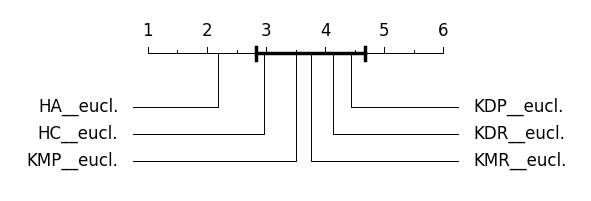
\includegraphics[width=\linewidth]{figuras/figure_combinacoes_1.png}
	\caption{Resultado do teste de Bonferroni-Dunn após o ranqueamento dos valores de VI. A estratégia de controle se ecnontra centrada no ranking médio da estratégia \emph{k-means(random)} com distância Euclidiana.}
	\label{fig:VIP1}
\end{figure}

\subsection{Métricas de dissimilaridade} \label{exp:2}

O objetivo deste segundo experimento é de comparar o desempenho
das diferentes métricas de dissimilaridade. Desde que o algoritmo exerce 
influência no desempenho individual da métrica, o procedimento usado 
neste experimento foi fixar o algoritmo de agrupamento 
e variar as métricas. O algoritmo fixado foi o agrupamento 
hierárquico com linkagem \emph{average}, por este ter apresentado o melhor 
resultado no experimento anterior. A combinação \emph{k-means} e 
distância Euclidiana foi também avaliada neste experimento, por se tratar 
da combinação padrão adotada na literatura. Todas as combinações 
deste experimento são mostradas na Tabela ~\ref{tbl:2}. 

%\begin{center}
	%\resizebox{\columnwidth}{!}{%
	\begin{table}		
	\centering
	\begin{tabular}{llllll}
		\toprule
		{} &              Id &             Algoritmo &      Similaridade \\
		\midrule
		0 &  HA\_\_cort-eucl. &  hierarchical-average &       cort-eucl. \\
		1 &         HA\_\_DTW &  hierarchical-average &        DTW \\
		2 &   HA\_\_cid-eucl. &  hierarchical-average &        cid-eucl. \\
		3 &      KMR\_\_eucl. &               k-means(random) &              eucl. \\
		4 &       HA\_\_eucl. &  hierarchical-average &         eucl. \\
		\bottomrule
	\end{tabular}
	%}
	%\captionof{table}{Estratégias comparadas no experimento 2.}  \label{tbl:2} 
	\caption{Estratégias comparadas no experimento 2.}  \label{tbl:2} 
		\end{table}
%\end{center}

Para $55$ bases de dados e $5$ combinações testadas, o valor crítico da estatística 
de Friedman é de $2.41$. A hipótese $H_0$ foi descartada, já que obteve-se $F_F=14.04$. Em seguida, 
deu-se prosseguimento ao teste \emph{post-hoc} de Bonferroni-Dunn, centrado na estratégia padrão (\emph{k-means(random)} com distância Euclidiana). O resultado, 
ilustrado na Figura ~\ref{fig:VIP2}, mostra que a combinação padrão é inferior à todas as demais, 
e além disso, que o uso da DTW e da CID acarretaram em melhoras significativas em relação à distância 
Euclidiana e CORT-Euclidiana. \\

\begin{figure}[h!]
	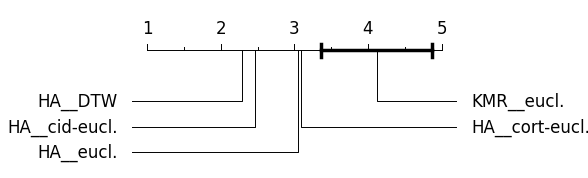
\includegraphics[width=\linewidth]{figuras/figure_combinacoes_2.png}
	\caption{Resultado teste Bonferroni-Dunn após o ranqueamento dos valores de VI, centrado no ranking médio da estratégia padrão (\emph{k-means(random)} com distância Euclidiana).}
	\label{fig:VIP2}
\end{figure}

\subsection{Comparação entre Métricas Promissoras} \label{exp:3}

Os experimentos anteriores mostraram que a adição de métricas 
robustas a distorções nos dados, tais como DTW e CID pode melhorar
significativamente a qualidade das partições obtidas. Com isso em mente, 
o objetivo deste experimento foi comparar as possíveis combinações 
envolvendo estas métricas promissoras nos quesitos de qualidade das 
partições (índice VI) e custo computacional (tempo de processamento). 
As combinações analisadas neste experimento se encontram na Tabela ~\ref{tbl:3}. 
Observe que, novamente, o algoritmo hierárquico com linkagem \emph{average} foi 
fixado.

%\begin{center}
	
	%	\resizebox{\columnwidth}{!}{%
	\begin{table}
		\centering		
	\begin{tabular}{llllll}
		\toprule
		{} &              Id &             Algoritmo & Similaridade \\
		\midrule
		0 &  HA\_\_cort-eucl. &  hierarchical-average & cort-eucl. \\
		1 &         HA\_\_DTW &  hierarchical-average &  DTW \\
		2 &   HA\_\_cid-eucl. &  hierarchical-average &  cid-ecul. \\
		3 &    HA\_\_cort-DTW &  hierarchical-average &  cort-DTW \\
		4 &     HA\_\_cid-DTW &  hierarchical-average &   cid-DTW \\
		\bottomrule
	\end{tabular}
	%	}
%	\captionof{table}{Estratégias do experimento 3.}  \label{tbl:3}
	\caption{Estratégias do experimento 3.}  \label{tbl:3}
		\end{table}
%\end{center}
%\setlength\parindent{20pt}

O teste de Friedman foi aplicado para testar a hipótese nula de que as estratégias 
são equivalentes. Para $55$ bases de dados e $5$ estratégias, o valor crítico 
é de $2.41$. Considerando o quesito tempo de processamento, 
obteve-se $F_F=543.03$ e, para o VI, $F_F=3.48$. Logo, 
para ambos os casos, a hipótese nula de que os rankings médios são iguais 
foi descartada. Deu-se então prosseguimento ao teste \emph{post-hoc} de Nemenyi, 
com o objetivo de verificar quais grupos de estratégias possuem desempenhos 
equivalentes. O diagrama resultante do teste de Nemenyi para o índice VI pode ser 
visto na Figura ~\ref{fig:VIP3}. O diagrama correlato, para o 
tempo de processamento, é mostrado na Figura ~\ref{fig:VIP4}. 

Pode-se concluir, com  base na Figura ~\ref{fig:VIP3}, que todas as combinações 
envolvendo as métricas DTW e CID são significamente melhores que a 
combinação envolvendo CORT e Euclidiana (HA\_cort-eucl.). 
A Figura ~\ref{fig:VIP4}, por sua vez, mostra que todas as combinações 
envolvendo DTW (HA-DTW, HA\_CID-DTW, HA\_cort-DTW) possuem maior custo computacional, 
sendo estatisticamente inferiores em relação as demais combinações. 
Uma análise conjunta, envolvendo os dois quesitos, apontam a combinação HA\_CID-eucl. 
como um bom equilíbrio entre a qualidade das partições obtidas e o menor tempo 
de processamento.

Com relação ao índice VI (Figura ~\ref{fig:VIP3}), observa-se ainda que, 
embora o teste não tenha apontado diferença estatística, os resultados 
em termos dos \textit{rankings} médios apontam que a correção CID (complexidade) 
produz efeito mais positivo do que a correção CORT (correlação temporal), 
independentemente da métrica convencional adotada: Euclidiana ou DTW. 
Além disso, todas as combinações envolvendo DTW se mostraram melhores 
que as outras em termos de \textit{rankings} médios, o que sugere a importância 
de um critério que seja invariante a deslocamentos locais no agrupamento 
de séries temporais.

\begin{figure}[h!]
	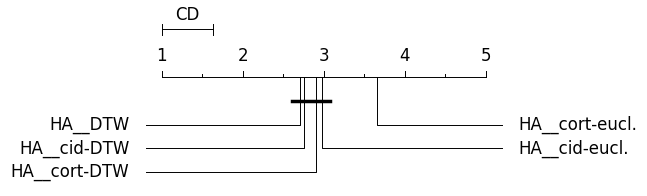
\includegraphics[width=\linewidth]{figuras/figure_combinacoes_4.png}	
	\caption{Resultado teste Nemenyi após o ranqueamento dos valores de VI.}
	\label{fig:VIP3}
\end{figure}

\begin{figure}[h!]	
	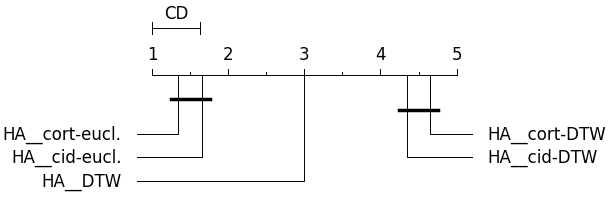
\includegraphics[width=\linewidth]{figuras/figure_combinacoes_3.png}
	\caption{Resultado teste Nemenyi após o ranqueamento dos valores de tempo de processamento.}
	\label{fig:VIP4}
\end{figure}


\section{Segundo experimento - Índice de validação interno} \label{sec:definicao_indice_interno}

Neste segundo experimento, tentaremos responder às seguintes perguntas:

\begin{itemize}
	\item Existe algum índice de validação interno que seja mais adequado para a definição do número de grupos um conjunto de dados de séries temporais?
	\item Uma vez definido o número de grupos, existe algum índice interno que seja mais indicado para avaliar as partições obtidas por diferentes estratégias de agrupamento?
\end{itemize}

Para responder à ambas perguntas os índices internos exibidos na Tabela ~\ref{tbl:indices_internos} foram comparados nos experimentos desta seção. Além desses índices da tabela, outros três índices farão parte da análise. Eles derivam da combinação de todos os índices da tabela, denominados índices puros, e são definidos como a moda (ou voto majoritário), média e mediana do número de grupos indicado por cada um dos $7$ índices.

\begin{center} 
	\begin{table}
		\caption{Principais índices internos de validação disponíveis na literatura}  \label{tbl:indices_internos}
		\resizebox{\columnwidth}{!}{%
			\begin{tabular}{lllll}
				\hline\noalign{\smallskip}
				Índice & Notação & Definição & Valor ótimo & Ref.\\
				\noalign{\smallskip}
				\hline
				\noalign{\smallskip}
				Calinski-Harabasz & CH & $\frac{\sum_i{n_i d^2(c_i,c)/(k-1)}}{\sum_i\sum_{x \in C_i} d^2(x,c_i)/(n-k) }$ & Max & \cite{CH} \\
				I index& I & $\bigg( \frac{1}{k} . \frac{\sum_{x \in X} d(x,c)}{\sum_i\sum_{x \in C_i} d(x,c_i)} . max_{i,j} d(c_i,c_j)\bigg)^p$ & Max & \cite{I}\\
				Dunn's index & Dunn & $min_i\bigg(min_j\bigg( \frac{min_{x \in C_i, y \in C_j} d(x,y))}{max_k(max_{x,y \in C_k} d(x,y))} \bigg)\bigg)$ & Max & \cite{Dunn} \\
				Silhouette & silhouette & $\frac{1}{k} . \sum_i^k \frac{1}{n_i} \sum_{x \in C_i} \frac{b(x)-a(x)}{max(b(x),a(x))}$ & Max & \cite{silhouette}\\
				Davies-Bouldin & DB & $\frac{1}{k} \sum_i max_{j,j \neq i} \bigg( \bigg( \frac{1}{n_i} \sum_{x \in C_i} d(x,c_i) + \frac{1}{n_j} \sum_{x \in C_j} d(x,c_j) \bigg) / d(c_i,c_j) \bigg)$ & Min & \cite{DBI}\\
				Xie-Beni & XB & $\frac{\sum_i \sum_{x \in C_i} d^2(x,c_i)}{n.min_{i,j \neq i} d^2(c_i,c_j)}$ & Min & \cite{XB}\\
				SD validity & SD & $Dis(k_{max}) Scat(k) + Dis(k)$ & Min & \cite{SD}\\
				{} & {} & $Scat(k) = \frac{1}{k} \frac{\sum_i^k ||\sigma(C_i)||}{||\sigma(X)||}$ & {} & {}\\
				{} & {} & $Dis(k) = \frac{max_{i,j}d(c_i,c_j)}{min_{i,j, i \neq j}d(c_i,c_j)} \sum_i^k \big( \sum_{j,j \neq i}^k d(c_i,c_j)  \big)^{-1}$ & {} & {}\\
				\hline
			\end{tabular}
		}
	\end{table}
\end{center}  

Na Tabela ~\ref{tbl:indices_internos} se encontram os índices internos a serem utilizados nesta seção,  onde $X$: é todo o conjunto de dados; $c$: é o centróide (quando a métrica de dissimilaridade escolhida é a distância euclidiana) ou medóide de $X$; $C_i$: $i$-ésimo grupo;  $n_i$: número de instâncias no $i$-ésimo grupo; $c_i$: centróide ou medóide do $i$-ésimo grupo; 
$d(x,y)$: medida de dissimilaridade entre $x$ e $y$; $n$: número de elementos em $X$; $k$: número de grupos em $X$, $||v|| = (v^T.v)^{\frac{1}{2}}$ e $\sigma(C_i)$: vetor de variância de todas as instâncias contidas em $C_i$; 
$p$: valor inteiro, recomendado $p=2$ ~\parencite{I}, $b(i)$: a menor dissimilaridade média da instância $i$ e cada instância contida em grupos diferentes do grupo de $i$ ;  $a(i)$ é a média de dissimilaridade da instância $i$ para todas as outras instâncias contidas no mesmo grupo de $i$.

\subsection{Índice para a definição do número de grupos} \label{sec:indice_iterativo}

Em tarefas de agrupamento, quando não se sabe \emph{a priori} o número de grupos nos quais os dados se encontram naturalmente divididos, são necessárias estratégias para se definir este número, já que ele é o principal parâmetro de entrada dos algoritmos particionais como o \emph{k-means} e o \emph{k-medoids}. Mesmo para algoritmos hierárquicos, esta é uma informação importante, pois a interpretação dos dendrogramas muitas vezes não é trivial, já que é difícil a definição do ponto de corte da árvore que define o particionamento dos dados. 

Uma estratégia comum é realizar diversos agrupamentos para diferentes valores de $k$ (número de grupos), dentro de determinado intervalo, no qual se espera que o valor ótimo $k_{opt}$, ou real, de grupos se encontra. Após a avaliação de cada partição resultante por um índice de validação interno, aquela que possuir um valor mais próximo do valor ótimo do índice, será a partição que apresenta o número ótimo ou mais indicado de grupos dentro do intervalo testado.

Dessa maneira, surge a pergunta: qual, ou quais, dos índices internos detalhados na literatura são mais interessante para a tarefa de se definir o número de agrupamentos de um conjunto de dados de séries temporais? Para responder à essa pergunta, iremos utilizar, novamente, o conjunto de dados UCR \emph{Time series} ~\parencite{UCRArchive}. Como cada conjunto de dados se encontra rotulado é sabido \emph{a priori} o número de grupos que os dados se encontram divididos em cada conjunto de dados. Assim, dado o valor esperado de determinado conjunto de dados, denominado $k_{opt}$, foi formado um intervalo $k = k_{opt}-6,k_{opt}-5,...,k_{opt},...,k_{opt}+6$, onde caso o primeiro valor seja menor que $2$, o intervalo é definido, necessariamente, a partir deste valor, já que em tarefas de agrupamento não faz sentido um valor de $k$ menor do que $2$.

Após a escolha de um algoritmo e uma métrica de dissimilaridade como, por exemplo, um algoritmo de agrupamento hierárquico com linkagem \emph{average} e a métrica CID-euclidiana, para cada valor de $k$ no intervalo criado, uma partição é obtida e avaliada com cada um dos índices da Tabela ~\ref{tbl:indices_internos}. A título de exemplo, tal procedimento, com o algoritmo e métrica de dissimilaridade acima mencionado, foi realizado no conjunto de dados \emph{Herring} (vide Figura ~\ref{fig:Herring}), que possui $k_{opt}=2$, e os resultados podem ser vistos na Tabela ~\ref{tbl:indices_iterativos}. Os índices DBI, XB e silhouette tiveram êxito na sugestão do valor de $k_{opt}$, ao passo que todos os demais falharam em tal tarefa. A partir da combinação da sugestão de cada um dos $7$ índices testados podem-se derivar os seguintes índices: moda dos valores sugeridos, cujo valor é 2; média dos valores sugeridos, que possui valor $3.57$ que é truncado para $4$ já que este é o valor inteiro mais próximo; e finalmente mediana dos valores sugeridos para $k_{opt}$, cujo valor é 3. Logo, para o teste em questão, dentre os índices originados pela combinação dos índices puros, somente a moda teve sucesso na indicação do valor de $k_{opt}$.

\begin{table} []
	\centering
	\caption{Resultados dos experimentos iterativos para o conjunto de dados \emph{Herring}, cujo número de grupos é igual a 2. Os valores em negrito representam os melhores valores obtidos em cada índice.}  \label{tbl:indices_iterativos}
%	\resizebox{\columnwidth}{!}{%
		\begin{tabular}{lrrrrrrrr}
			\toprule
			{} &    k &      CH &    DBI &   Dunn &       I &     SD &     XB &  silhouette \\
			\midrule
   \rowcolor{lightgray} &  2.0 &   2.025 &  \bfseries{0.486} &  0.369 &   0.031 &  0.517 &  \bfseries{0.478} &       \bfseries{0.409} \\
   &  3.0 &  20.876 &  0.492 &  0.353 &  15.024 &  \bfseries{0.414} &  0.489 &       0.259 \\
   &  4.0 &  \bfseries{21.448} &  0.879 &  0.262 &  \bfseries{20.746} &  0.569 &  0.614 &       0.206 \\
   &  5.0 &  16.315 &  0.826 &  0.267 &  14.124 &  0.500 &  0.598 &       0.183 \\
   &  6.0 &  14.646 &  1.184 &  0.330 &  12.780 &  0.806 &  0.982 &       0.195 \\
   &  7.0 &  12.879 &  1.073 &  0.334 &  10.826 &  0.759 &  0.961 &       0.186 \\
   &  8.0 &  10.987 &  1.208 &  \bfseries{0.378} &   8.506 &  0.908 &  1.092 &       0.184 \\
			\bottomrule
		\end{tabular}
	%}
\end{table} 

Os valores em negrito na Tabela ~\ref{tbl:indices_iterativos} representam os melhores valores obtidos em cada índice, e quando este valor coincide com o valor de $k_{opt}$, então um acerto é computado para o índice naquela base. Em seguida, tal procedimento foi repetido para 70 bases de dados, com o objetivo de se construir uma tabela binária, representado os acertos e erros de cada índice em cada base. Ao final da tabela, o número de acertos de cada índice foi somado e dividido pelo número de bases, para se ter uma ideia da porcentagem de vezes que cada índice obteve sucesso. Devido às suas grandes dimensões (70x13), somente parte da tabela binária de tal experimento pode ser vista na Tabela ~\ref{tbl:indices_hits}, já que diversas linhas (datasets) e algumas colunas (índices) da tabela não se encontram presentes.

	\begin{table}[]
		\centering
		\caption{Resultados dos experimentos iterativos para cada conjunto de dados, onde o asterisco corresponde à um sucesso na sugestão do índice para a base de dados. Foi utilizado o algoritmo hierárquico com linkagem \emph{average} e métrica de dissimilaridade cid-euclidiana.}  \label{tbl:indices_hits} 
		%\resizebox{\columnwidth}{!}{
		%{\footnotesize
			\begin{tabular}{llrrrrrr}
				\toprule
				{} &                         Conjunto de dados &     CH &    DBI &   Dunn &      I &     SD &     XB \\
				\midrule
				0  &                         50words &    &    &    &    &    &   \\
				1  &                           Adiac &    &    &    &    &    &    \\
				2  &                       ArrowHead &  * &    &    &  * &    &  \\				
				26 &                         Herring &    &  * &    &    &    &  * \\			
				69 &                            yoga &  * &    &    &    &    &    \\
				 \rowcolor{lightgray} 70 &                           Total &  0.429 &  0.214 &  0.143 &  0.257 &  0.171 &  0.343\\
				 {} &                         {}  &     CH &    DBI &   Dunn &      I &     SD &     XB\\
			\bottomrule
		\end{tabular}
		%}
	\end{table}
	
	%	\begin{longtable}
	%	\caption{Resultados dos experimentos iterativos para cada conjunto de dados, onde o asterisco corresponde à um sucesso na sugestão do índice para a base de dados. Foi utilizado o algoritmo hierárquico com linkagem \emph{average} e métrica de dissimilaridade cid-euclidiana.}
	%\resizebox{\columnwidth}{!}{
	%{\footnotesize
	%	\begin{longtable}{llrrrrrrrrrr}
	%		\toprule
	%		{} &                         Conjunto de dados &     CH &    DBI &   Dunn &      I &     SD &     XB &  silhouette &  média &   moda &  mediana \\
	%		\midrule
	%		0  &                         50words &    &    &    &    &    &    &         &   * &    &      \\
	%		1  &                           Adiac &    &    &    &    &    &    &         &    &    &      \\
	%		2  &                       ArrowHead &  * &    &    &  * &    &    &         &    &    &      \\
	%	3  &                            Beef &    &    &    &    &    &    &         &   * &    &      \\
	%		4  &                       BeetleFly &  * &    &    &  * &    &    &         &    &    &      \\
	%		5  &                     BirdChicken &    &    &    &    &    &    &         &    &    &      \\
	%		6  &                             CBF &  * &    &    &  * &    &    &       * &    &  * &      \\
	%		7  &                             Car &    &    &    &    &    &    &         &    &    &      \\
	%		8  &           ChlorineConcentration &    &    &  * &    &    &    &         &   * &    &      \\
	%		9  &                          Coffee &  * &    &    &    &    &    &         &    &    &      \\
	%		10 &                       Computers &  * &    &    &    &  * &    &       * &    &  * &      \\
	%		11 &             DiatomSizeReduction &  * &    &    &    &    &    &         &    &    &      \\
	%		12 &    DistalPhalanxOutlineAgeGroup &  * &  * &    &  * &    &  * &       * &   * &  * &     * \\
	%		13 &     DistalPhalanxOutlineCorrect &    &  * &  * &    &  * &  * &       * &    &  * &     * \\
	%		14 &                 DistalPhalanxTW &    &    &    &    &    &    &         &    &    &      \\
	%		15 &                          ECG200 &  * &  * &    &  * &    &  * &       * &    &  * &     * \\
	%		16 &                         ECG5000 &  * &    &    &  * &    &    &         &    &    &      \\
	%		17 &                     ECGFiveDays &  * &    &    &    &    &  * &         &    &  * &      \\
	%		18 &                     Earthquakes &    &  * &  * &    &    &  * &       * &    &  * &     * \\
	%		19 &                            FISH &    &    &    &    &    &    &         &    &    &      \\
	%		20 &                         FaceAll &    &    &    &    &    &    &         &    &    &    \\
	%		21 &                        FaceFour &    &    &    &    &  * &    &         &    &    &      \\
	%		22 &                        FacesUCR &    &    &    &    &    &    &         &    &    &      \\
	%		23 &                           FordB &  * &    &    &  * &    &  * &       * &    &  * &     * \\
	%		24 &                       Gun\_Point &  * &  * &  * &  * &  * &  * &       * &   * &  * &     * \\
	%		25 &                             Ham &    &  * &  * &    &  * &  * &       * &   * &  * &     * \\
	%		26 &                         Herring &    &  * &    &    &    &  * &       * &    &  * &      \\
	%		27 &             InsectWingbeatSound &    &    &    &    &    &    &         &    &    &      \\
	%		28 &                ItalyPowerDemand &  * &    &    &    &  * &  * &       * &    &  * &     * \\
	%		29 &          LargeKitchenAppliances &    &    &    &    &    &    &         &    &    &      \\
	%		30 &                       Lighting2 &  * &  * &    &  * &  * &  * &       * &   * &  * &     * \\
	%		31 &                       Lighting7 &    &    &    &    &    &    &         &    &    &      \\
	%		32 &                            Meat &  * &    &  * &  * &  * &  * &       * &   * &  * &     * \\
	%		33 &                   MedicalImages &    &    &    &    &    &    &         &    &    &      \\
	%		34 &    MiddlePhalanxOutlineAgeGroup &  * &    &    &  * &    &  * &       * &   * &  * &     * \\
	%		35 &     MiddlePhalanxOutlineCorrect &  * &    &  * &    &    &  * &       * &    &  * &     * \\
	%		36 &                 MiddlePhalanxTW &    &    &    &    &    &    &         &    &    &      \\
	%		37 &                      MoteStrain &  * &  * &    &  * &  * &  * &       * &   * &  * &     * \\
	%		38 &                         OSULeaf &    &    &    &    &    &    &         &    &    &      \\
	%		39 &                        OliveOil &    &    &    &    &    &    &         &    &    &      \\
	%		40 &                           Plane &    &    &    &    &    &    &         &    &    &      \\
	%		41 &  ProximalPhalanxOutlineAgeGroup &    &    &    &    &    &    &         &   * &    &      \\
	%		42 &   ProximalPhalanxOutlineCorrect &    &    &    &    &    &    &       * &    &    &      \\
	%		43 &               ProximalPhalanxTW &    &    &    &    &    &    &         &    &    &      \\
	%		44 &            RefrigerationDevices &  * &    &    &    &    &    &         &   * &    &      \\
	%		45 &                      ScreenType &    &    &    &    &    &    &         &    &    &      \\
	%		46 &                     ShapeletSim &  * &  * &    &  * &    &    &         &    &    &      \\			
	%		47 &                       ShapesAll &    &    &    &    &    &    &         &    &    &      \\
	%		48 &          SmallKitchenAppliances &    &    &    &    &    &    &         &   * &    &      \\
	%		49 &            SonyAIBORobotSurface &  * &    &  * &  * &    &  * &       * &    &  * &     * \\
	%		50 &          SonyAIBORobotSurfaceII &  * &    &    &  * &    &    &         &    &    &      \\
	%		51 &                      Strawberry &  * &  * &    &    &    &  * &       * &    &  * &     * \\
	%	52 &                     SwedishLeaf &    &    &    &    &    &    &         &    &    &      \\
	%		53 &                         Symbols &    &    &    &    &    &    &         &    &    &      \\
	%	54 &                ToeSegmentation1 &  * &    &    &    &    &  * &       * &    &  * &      \\
	%		55 &                ToeSegmentation2 &  * &    &    &  * &    &    &       * &    &  * &      \\
	%		56 &                           Trace &    &    &    &    &    &    &         &    &    &      \\
	%		57 &                      TwoLeadECG &  * &    &    &    &  * &  * &       * &    &  * &     * \\
	%	58 &                    Two\_Patterns &    &    &    &    &    &    &         &    &    &      \\
	%		59 &          UWaveGestureLibraryAll &    &    &    &    &    &    &         &    &    &      \\
	%		60 &                            Wine &    &  * &  * &    &    &  * &       * &    &  * &     * \\
	%		61 &                   WordsSynonyms &    &    &    &    &    &    &         &    &    &      \\
	%		62 &                           Worms &    &    &    &    &    &    &         &    &    &      \\
	%		63 &                   WormsTwoClass &    &  * &    &    &  * &  * &       * &    &  * &     * \\
	%		64 &                 easy\_clustering &  * &  * &  * &  * &  * &  * &       * &   * &  * &     * \\
	%		65 &                             foo &  * &    &    &  * &    &  * &       * &    &  * &     * \\
	%		66 &                     synthetic\_6 &    &    &    &    &    &    &         &    &    &      \\
	%		67 &               synthetic\_control &    &    &    &    &    &    &         &    &    &      \\
	%		68 &                           wafer &  * &  * &    &    &    &  * &       * &    &  * &     * \\
	%		69 &                            yoga &  * &    &    &    &    &    &         &    &    &      \\
	%		\rowcolor{lightgray} 70 &                           Total &  0.429 &  0.214 &  0.143 &  0.257 &  0.171 &  0.343 &       0.386 &   0.2 &  0.386 &     0.3 \\
	%		{} &                         {}  &     CH &    DBI &   Dunn &      I &     SD &     XB &  silhouette &  média &   moda &  mediana \\
	%		\bottomrule
%		\end{longtable}\label{tbl:indices_hits} 
%	}
	%}
	%\end{longtable} \label{tbl:indices_iterativos} 

O total da tabela binária obtida pela combinação do algoritmo hierárquico com linkagem \emph{average} e métrica de dissimilaridade cid-euclidiana foi armazenado, assim como os totais obtidos por diversas outras combinações. Com todos os totais, obtidos por diferentes combinações de algoritmos de agrupamento e métricas de dissimilaridade, pôde-se formar uma terceira tabela, cuja as linhas são compostas pelas diferentes combinações de algoritmo e métrica de dissimilaridade, enquanto as colunas são os índices, puros e combinados, utilizados na tarefa iterativa de se apontar o número de agrupamentos. Os valores de tal tabela contêm cada um a porcentagem de vezes que um índice aponta corretamente o número de agrupamentos de um conjunto de dados de séries temporais para determinada combinação de métrica de dissimilaridade e algoritmo de agrupamento. 

A tabela resultante possui $78$ linhas, ou combinações de algoritmos e métricas de dissimilaridade, e $10$ colunas, ou índices testados, o que faz com que o valor crítico para o teste não-paramétrico de Friedman seja $F_{crit} = 1.79$, para uma significância de 5\%. Após a obtenção do ranking médio de cada índice e a realização do teste de Friedman, obteve-se o valor $F_F = 258.42$, o que descarta a hipótese nula $H_0$ de que os índices possuem performance equivalente frente às diferentes estratégias testadas. Dessa maneira, deu-se prosseguimento ao teste \emph{pos-hoc} de Nemenyi, para verificar se existe algum índice, ou grupo de índices, que possua performance superior aos demais. O resultado do teste de Nemenyi pode ser visto na Figura ~\ref{fig:resultado_iterativo}, onde se destaca o o grupo de índices formado pelo Calinski-Harabasz e a moda da sugestão de todos os índices, já que este grupo possui um ranking médio menor do que os demais gruposs.

Logo, conclui-se que o índice Calinski-Harabasz é o mais indicado para a tarefa de se definir o número de grupos em que um conjunto de dados de séries temporais se encontra naturalmente dividido, já que para a obtenção do índice combinado moda, que possui performance equivalente, faz-se necessária a obtenção de todos os demais índices puros além do citado índice, o que, do ponto de vista do custo computacional, não é interessante.

 \begin{figure}
 	%\vspace{2.5cm}
 	%\resizebox{\columnwidth}{!}
 	\caption{Resultado do teste de Nemenyi para o teste do melhor índice interno para apontar o número de grupos.}
 \end{figure} \label{fig:resultado_iterativo}


\subsection{Índice interno para avaliação de partições com o número de grupos definido} \label{sec:indice_interno_k_fixo}

Uma vez definido o número de grupos, surge outra pergunta: qual dos índices internos da Tabela ~\ref{tbl:indices_internos} é o mais indicado para avaliar a qualidade de diferentes partições? Ou, em outras palavras, qual índice interno é o melhor indicador que houve uma melhora, ou piora, na partição resultante após uma alteração nos parâmetros ou estratégias de agrupamento com exceção do número de grupos? Nos experimentos será utilizada a distância de kendall-tau que é uma medida de dissimilaridade entre dois rankings e definida como a contagem do número de discordâncias entre os dois rankings em análise ~\parencite{kendall_tau}. Vale ressaltar que a medida de Kendall-tau, que varia no intervalo $[-1,1]$, é uma métrica no espaço de rankings, de forma que valores maiores implicam em rankings mais próximos. Quando dois rankings são idênticos, o valor da métrica Kendall-Tau entre eles é 1.

Com o objetivo de elucidar a proposta deste experimento, foi realizado o seguinte experimento:
\begin{itemize}
	\item escolheu-se arbitrariamente uma base de dados do UCR \emph{Time Series} (\emph{synthetic_control} que possui 6 grupos, vide Figura ~\ref{fig:synthetic_control}),
	\item escolheu-se arbitrariamente uma métrica de dissimilaridade (distância Euclidiana),
	\item realizou-se seis agrupamentos do conjunto de dados com os seguintes algoritmos: \emph{hierarchical-average (HA), hierarchical-complete (HC), hierarchical-single (HS), k-means++ (KP), k-means (KR), k-medoids(PAM)(KP)},
	\item avaliou-se cada uma das seis partições obtidas com os seguintes índices: VI, silhouette, Calinski-Harabasz.
\end{itemize}

Os resultados numéricos podem ser vistos na Tabela ~\ref{tbl:rankings_3}, bem como os valores ranqueados na Tabela ~\ref{tbl:rankings}. Em seguida, calculou-se a distância Kendall-Tau entre o ranking do índice silhouette e o ranking do índice VI, onde obteve-se o valor -0.20, bem como a distância Kendall-Tau entre o ranking do índice Calinski-Harabasz e o ranking do índice VI, onde obteve-se o valor 0.33. Logo, como valores maiores de Kendall-Tau implicam em rankings mais coerentes entre si, pode-se afirmar que o índice Calinski-Harabasz, ao se variar o algoritmo de agrupamento, na base de dados e métrica de dissimilaridade escolhidas, tem comportamento, no que diz respeito a indicar uma piora ou melhora da partição, mais similar ao índice VI do que o índice silhouette.

A partir deste breve experimento, pode-se afirmar que, caso não se tivesse disponível a rotulação dos dados, mas somente o número de grupos, o índice Calinski-Harabasz é mais indicado que o índice silhouette para indicar uma melhora, ou piora, nas partições obtidas com a variação do algoritmo de agrupamento para a base de dados e métrica de dissimilaridade escolhida.

%\begin{center}
	\begin{table}[]
		\centering
		\caption{Rankings dos valores dos índices Para cada uma das partições obtidas variando-se o algoritmo de agrupamento.} 	\label{tbl:rankings_3}
		\begin{tabular}{lrrrrrr}
			\toprule
			{} &          HC &          HA &         HS &          KM &          KR &          KP \\
			\midrule
			VI &   1.41 &   1.39 &  1.84 &   0.84 &   0.73 &   2.57 \\
			Calinski-Harabasz &  42.04 &  49.11 &  1.02 &  55.73 &  55.87 &  26.27 \\
			silhouette &   0.23 &   0.25 & -0.01 &   0.21 &   0.21 &  -0.01 \\
			\bottomrule
		\end{tabular}
			\end{table}
%\end{center}

%\begin{center}
	\begin{table}[]
		\centering
		\caption{Rankings dos valores dos índices da tabela ~\ref{tbl:rankings_3}. Note que valores maiores para o Calinski-Harabasz e o silhouette implicam em rankings melhores, ao passo que para o VI em rankings piores.} 	\label{tbl:rankings}
		\begin{tabular}{lrrrrrr}
			\toprule
			{} &          HC &          HA &         HS &          KM &          KR &          KP \\			
			\midrule
			VI &  5 &  4 &  2 &  1 &  3 &  6 \\
			Calinski-Harabasz &  5 &  4 &  2 &  1 &  6 &  3 \\
			silhouette &  2 &  1 &  5 &  4 &  6 &  3 \\
			\bottomrule
		\end{tabular}
	\end{table}

%\end{center}

O experimento realizado restringiu-se a uma base  de dados, à dois índices internos e à avaliação da variação do algoritmo de agrupamento. Para realizar um estudo mais amplo, foram realizados agrupamentos com um pequeno grupo de $55$ combinações de algoritmo de agrupamento e métrica de dissimilaridade e de $71$ conjuntos de dados de séries temporais, novamente conjuntos de dados do UCR \emph{Time Series} ~\parencite{UCRArchive}. Cada partição obtida foi avaliada por cada um dos índices internos da Tabela ~\ref{tbl:indices_internos} e pelo índice externo VI exposto na seção ~\ref{sec:VI}. Como o VI é uma métrica no espaço de partições, uma melhora ou piora no seu valor indica uma respectiva melhora ou piora na aproximação da partição real em função de uma estratégia de agrupamento melhor ou pior para determinada base de dados. Dessa maneira, espera-se que os índices internos que acompanharem a melhora ou piora do VI em função das variações da estratégia de agrupamento sejam os mais indicados para avaliar partições com o número de grupos definido. 

Para se comparar a aderência, ou coerência, de cada índice interno ao VI, todos os índices para cada base foram ranqueados em função das estratégias escolhidas. Em seguida, para cada base e para cada índice foi calculada a distância de Kendall-Tau entre os rankings obtidos pelo VI e os rankings obtidos para cada índice. Os resultados podem ser vistos na Tabela ~\ref{tbl:coherence}, que contêm os valores $1-\tau$, onde $\tau$ é o valor Kendall-Tau, de forma que valores menores indicam uma maior coerência do índice interno com o índice VI.

\begin{longtable}{llllllll}
	\caption{Tabela com os valores de Kendall-Tau dos índices em relação ao VI.}
	 \label{tbl:coherence}\\
	% \endfirsthead
%	 \endhead
	\toprule
	{} &                         dataset &    CH &   DBI & silhouette &    SD &    XB &  Dunn \\
	\midrule
	0  &                         50words &  0.91 &  1.13 &       0.91 &  1.24 &  1.08 &  0.93 \\
	1  &                           Adiac &  0.98 &  0.68 &       1.03 &  0.92 &  0.74 &  1.08 \\
	2  &                       ArrowHead &  1.04 &  0.95 &       0.78 &  1.14 &  1.02 &  1.01 \\
	3  &                       BeetleFly &  0.87 &  1.11 &       1.11 &  1.11 &  1.29 &  0.97 \\
	4  &                             CBF &  1.11 &  1.15 &       0.74 &  0.84 &  1.05 &  0.92 \\
	5  &                             Car &  1.07 &  1.02 &       0.95 &  0.96 &  1.07 &  0.84 \\
	6  &           ChlorineConcentration &  1.08 &  1.08 &       0.66 &  1.09 &  0.98 &  0.81 \\
	7  &                  CinC\_ECG\_torso &  0.85 &  0.94 &       0.79 &  1.17 &  1.00 &  0.78 \\
	8  &                          Coffee &  0.82 &  1.08 &       0.81 &  1.00 &  0.99 &  1.09 \\
	9  &                       Computers &  1.02 &  1.06 &       0.97 &  1.15 &  1.08 &  0.79 \\
	10 &             DiatomSizeReduction &  0.68 &  1.11 &       0.58 &  1.21 &  1.19 &  0.60 \\
	11 &    DistalPhalanxOutlineAgeGroup &  1.08 &  0.87 &       0.66 &  0.91 &  0.93 &  0.82 \\
	12 &     DistalPhalanxOutlineCorrect &  1.34 &  1.44 &       0.53 &  1.01 &  1.40 &  0.69 \\
	13 &                 DistalPhalanxTW &  1.01 &  1.17 &       0.92 &  0.90 &  1.11 &  0.92 \\
	14 &                          ECG200 &  1.14 &  1.19 &       0.63 &  1.02 &  1.15 &  0.77 \\
	15 &                         ECG5000 &  1.17 &  1.07 &       0.69 &  1.02 &  1.16 &  0.96 \\
	16 &                     ECGFiveDays &  1.16 &  1.05 &       1.24 &  0.85 &  0.77 &  1.26 \\
	17 &                     Earthquakes &  1.03 &  0.79 &       0.86 &  1.19 &  0.84 &  1.03 \\
	18 &                            FISH &  1.07 &  1.07 &       0.76 &  0.95 &  1.23 &  0.90 \\
	19 &                        FaceFour &  1.01 &  1.10 &       0.93 &  1.12 &  1.07 &  1.00 \\
	20 &                        FacesUCR &  1.13 &  1.01 &       0.82 &  0.94 &  1.08 &  0.99 \\
	21 &                           FordA &  1.07 &  0.98 &       1.03 &  1.17 &  0.93 &  0.83 \\
	22 &                           FordB &  0.72 &  0.78 &       1.12 &  1.04 &  0.88 &  0.82 \\
	23 &                             Ham &  1.49 &  1.48 &       0.66 &  1.10 &  1.41 &  0.61 \\
	24 &                    HandOutlines &  1.32 &  1.27 &       0.61 &  1.03 &  1.27 &  0.61 \\
	25 &                         Haptics &  1.22 &  1.22 &       0.95 &  0.95 &  1.31 &  0.81 \\
	26 &                         Herring &  1.31 &  1.38 &       0.76 &  0.97 &  1.35 &  0.73 \\
	27 &                     InlineSkate &  1.13 &  1.30 &       0.65 &  0.98 &  1.23 &  1.01 \\
	28 &                ItalyPowerDemand &  0.95 &  1.20 &       0.84 &  1.15 &  1.12 &  0.82 \\
	29 &          LargeKitchenAppliances &  1.04 &  0.88 &       0.92 &  0.84 &  0.93 &  0.72 \\
	30 &                       Lighting2 &  0.89 &  1.11 &       0.88 &  0.81 &  1.16 &  0.93 \\
	31 &                       Lighting7 &  0.96 &  1.04 &       0.87 &  1.02 &  1.21 &  0.83 \\
	32 &                          MALLAT &  0.81 &  0.94 &       0.92 &  0.99 &  1.01 &  1.10 \\
	33 &                            Meat &  0.85 &  1.30 &       0.68 &  1.03 &  1.25 &  0.69 \\
	34 &                   MedicalImages &  1.06 &  1.11 &       0.80 &  1.01 &  1.03 &  0.72 \\
	35 &    MiddlePhalanxOutlineAgeGroup &  0.74 &  1.15 &       0.85 &  0.87 &  1.15 &  1.07 \\
	36 &     MiddlePhalanxOutlineCorrect &  1.12 &  1.10 &       0.96 &  0.90 &  0.93 &  0.41 \\
	37 &                 MiddlePhalanxTW &  1.17 &  1.38 &       0.83 &  0.84 &  1.19 &  0.64 \\
	38 &                      MoteStrain &  0.73 &  0.75 &       1.10 &  1.09 &  0.75 &  0.79 \\
	39 &     NonInvasiveFatalECG\_Thorax1 &  0.93 &  1.02 &       0.96 &  1.05 &  0.89 &  0.98 \\
	40 &     NonInvasiveFatalECG\_Thorax2 &  1.07 &  0.92 &       0.85 &  0.89 &  0.76 &  1.03 \\
	41 &                         OSULeaf &  1.03 &  1.15 &       0.82 &  0.77 &  1.04 &  0.99 \\
	42 &        PhalangesOutlinesCorrect &  1.37 &  1.40 &       0.86 &  1.30 &  1.30 &  0.74 \\
	43 &                         Phoneme &  0.94 &  1.04 &       0.84 &  1.20 &  1.03 &  1.06 \\
	44 &                           Plane &  0.84 &  1.02 &       0.74 &  1.14 &  1.06 &  0.85 \\
	45 &  ProximalPhalanxOutlineAgeGroup &  0.98 &  1.01 &       0.59 &  1.18 &  0.96 &  0.75 \\
	46 &   ProximalPhalanxOutlineCorrect &  1.05 &  0.72 &       1.01 &  1.12 &  0.95 &  0.87 \\
	47 &               ProximalPhalanxTW &  0.96 &  1.07 &       0.79 &  1.17 &  1.00 &  0.71 \\
	48 &            RefrigerationDevices &  1.11 &  1.18 &       0.91 &  1.05 &  1.18 &  0.87 \\
	49 &                      ScreenType &  1.14 &  0.96 &       0.88 &  1.15 &  0.97 &  1.02 \\
	50 &                       ShapesAll &  0.64 &  1.10 &       1.00 &  0.99 &  0.86 &  0.88 \\
	51 &          SmallKitchenAppliances &  1.15 &  1.03 &       0.72 &  0.93 &  1.06 &  0.92 \\
	52 &            SonyAIBORobotSurface &  1.16 &  1.01 &       0.50 &  0.93 &  0.88 &  0.74 \\
	53 &          SonyAIBORobotSurfaceII &  0.81 &  0.94 &       0.95 &  1.07 &  1.12 &  0.87 \\
	54 &                 StarLightCurves &  0.72 &  0.87 &       0.75 &  1.12 &  1.16 &  1.11 \\
	55 &                      Strawberry &  1.08 &  1.08 &       0.48 &  0.83 &  1.03 &  0.90 \\
	56 &                     SwedishLeaf &  0.72 &  1.02 &       0.96 &  0.96 &  0.99 &  1.01 \\
	57 &                         Symbols &  0.66 &  1.08 &       0.65 &  0.94 &  1.24 &  0.82 \\
	58 &                ToeSegmentation1 &  0.82 &  1.14 &       1.31 &  1.23 &  1.13 &  0.87 \\
	59 &                ToeSegmentation2 &  0.88 &  0.98 &       1.12 &  0.98 &  1.04 &  1.13 \\
	60 &                           Trace &  0.83 &  0.81 &       0.86 &  0.92 &  0.93 &  1.16 \\
	61 &                      TwoLeadECG &  1.06 &  1.13 &       0.78 &  0.95 &  1.15 &  0.61 \\
	62 &                    Two\_Patterns &  0.97 &  1.14 &       0.90 &  1.12 &  0.96 &  0.89 \\
	63 &          UWaveGestureLibraryAll &  0.82 &  1.03 &       0.78 &  1.09 &  0.97 &  0.88 \\
	64 &                            Wine &  1.39 &  1.36 &       0.67 &  1.15 &  1.30 &  0.56 \\
	65 &                   WordsSynonyms &  0.93 &  1.14 &       0.82 &  0.90 &  1.25 &  0.97 \\
	66 &                           Worms &  0.86 &  1.12 &       0.74 &  0.96 &  1.08 &  1.05 \\
	67 &                   WormsTwoClass &  0.73 &  0.84 &       0.87 &  1.14 &  0.89 &  1.09 \\
	68 &               synthetic\_control &  1.15 &  1.01 &       0.58 &  0.88 &  1.09 &  0.85 \\
	69 &                           wafer &  1.08 &  1.16 &       0.80 &  0.94 &  1.02 &  0.94 \\
	70 &                            yoga &  0.89 &  0.99 &       0.66 &  1.10 &  1.01 &  0.85 \\
	\midrule
	 \rowcolor{lightgray}    &			Rankings médios & 3.58 & 4.42 & 2.16 & 3.91 & 4.23 & 2.67 \\
	 	\midrule
	 {} &                         {} &    CH &   DBI & silhouette &    SD &    XB &  Dunn \\
	\bottomrule
\end{longtable}

Para $70$ bases e $6$ índices internos, o valor crítico da estatística de Friedman é de $F_{crit}=2.12$, e como  para os rankings médios destacados na Tabela ~\ref{tbl:coherence} foi obtido o valor $F_F = 18.11$, então a hipótese nula $H_0$ de que todos os índices possuem aderências equivalentes ao índice VI foi descartada. A partir desse resultado, deu-se prosseguimento ao teste de Nemenyi para verificar qual, ou quais, índice interno possui aderência significativamente maior que os demais índices. Os resultados podem ser vistos na Figura ~ \ref{fig:coherence}, que mostram que os índices silhouette e Dunn, possuem melhor aderência ao VI que os demais índices internos.

Logo, em uma tarefa de agrupamento real, no qual não se possui a rotulação dos dados e já se decidiu, ou já se sabe \emph{a priori}, o número de grupos que os dados se encontram divididos, os índices silhouette e Dunn são os mais indicados para avaliar as novas partições obtidas por diferentes estratégias de agrupamento.

 \begin{figure}
 	%\vspace{2.5cm}
 	%\resizebox{\columnwidth}{!}
 	\caption{Resultado do teste de Nemenyi para o teste de coerência dos índices internos com o VI.}
 \end{figure} \label{fig:coherence}

\section{Conclusões do Capítulo}

Os experimentos deste Capítulo buscaram definir uma estratégia padrão de agrupamento de séries temporais, e as estratégias testadas foram confrontadas com a estratégia padrão, que consiste na realização do agrupamento pelo algoritmo \emph{k-means} e distância Euclidiana. Dessa maneira, foram realizados dois experimentos, sendo o primeiro para estudar as influências da escolha do algoritmo e métrica de dissimilaridade na qualidade da partição de dados de séries temporais, enquanto o segundo experimento teve como objetivo estudar os índices de validação interna na avaliação das partições resultantes do agrupamento de séries temporais.

Assim, no primeiro experimento, foram realizados dois testes:
\begin{itemize}
	\item no primeiro foram testados diversos algoritmos de agrupamento fixando-se a distância Euclidiana como métrica de dissimilaridade e verificou-se a superioridade do algoritmo hierárquico com \emph{linkagem average},
	\item já no segundo teste, fixou-se o algoritmo de agrupamento, como o algoritmo hierárquico com \emph{linkagem average}, e variou-se as dissimilaridades. onde  verificou-se a superioridade da performance das dissimilaridades DTW e CID-Euclidiana em relação às demais dissimilaridades testadas.
\end{itemize}

No segundo experimento, também foram realizados dois testes:
\begin{itemize}
	\item no primeiro, os índices de validação interna foram testados para indicar aquele que é o mais adequado para a tarefa de apontar o número de grupos que as instâncias do conjunto de dados se encontram naturalmente divididas, e, após a análise dos resultados, chegou-se a conclusão que o índice Calinski-Harabasz é o mais indicado para tal,
	\item no segundo teste, procurou-se encontrar um índice da validação interna que seja mais coerente com o VI e, dessa maneira, um índice que seja um melhor indicador da melhora ou piora da partição dos dados de séries temporais ao se alterar a estratégia de agrupamento, chegou-se a conclusão que os índices Dunn e silhouette são os índices mais coerentes com o VI.
\end{itemize}

Dessa maneira, partindo-se do pressuposto que não se possui, \emph{a priori}, nenhuma informação útil para a realização do agrupamento, como, por exemplo, o número de grupos que as instâncias se encontram naturalmente divididas, os experimentos realizados em bases de dados rotuladas sugerem a seguinte abordagem a ser realizada no agrupamento de séries temporais:

\begin{itemize}
	\item Realizar algum tipo de normalização das curvas. Sugere-se a normalização Z ou normalização max.
	\item Escolher alguma medida de dissimilaridade. Sugere-se a CID-DTW caso o conjunto de dados não seja muito grande, ou os recursos computacionais escassos. Em qualquer uma dessas duas hipóteses, sugere-se a utilização da CID-Euclidiana.
	\item Para se definir o número de grupos $k$, realizar o agrupamento do conjunto de dados já normalizados pelo algoritmo hierárquico com \emph{linkagem average} e medida de dissimilaridade escolhida. Em seguida, obter diferentes partições a partir da poda do dendrograma obtido por valores iterativos de $k$, em um intervalo no qual se espera que se encontre o valor de $k$.
	\item Em seguida, para cada uma das partições obtidas, realizar a avaliação de cada uma delas pelo índice Calinski-Harabasz, e aquela que possuir o melhor valor indicará o valor de $k$.
	\item Caso se deseje realizar um refinamento da partição obtida até o momento, uma vez definido o número de grupos $k$, pode-se realizar outras partições com diferentes escolhas de combinações de algoritmos e métricas de dissimilaridade e avaliá-las pelo índice silhouette. A partição que acarretar no melhor valor do índice é a partição final da tarefa de agrupamento.
\end{itemize}

A estratégia descrita foi empregada no estudo de caso do Capítulo ~\ref{cap:estudo_de_caso}. Vale destacar que esta estratégia não garante resultados ótimos, ela é apenas uma sugestão inicial quando não se dispõe de informações relevantes para o agrupamento acerca dos dados. Nos próprios dados sintéticos do UCR \emph{Time Series}, verificou-se que para alguns conjuntos de dados em específico, a metologia proposta teve performance inferior à performance da estratégia padrão (\emph{k-means} com distância Euclidiana). No entanto, na média, levando-se em conta todos os conjuntos, os testes estatísticos demonstraram que ela é significativamente superior às demais estratégias, como a estratégia padrão, por exemplo.



 %Mesmo para outros algoritmos de agrupamento, baseados em densidade por exemplo, como o DBSCAN, que fazem uso de outros parâmetros que não o número de agrupamentos, os índices de validação são importantes. Em ~\parencite{DE_DBSCAN}, por exemplo, é proposto um algoritmo de evolução diferencial para escolher os melhores parâmetros do DBSCAN, e a função objetivo deste problema de otimização é baseada em índices de validação interna.






